\documentclass{article}
\usepackage[utf8]{inputenc}    
\usepackage[T1]{fontenc}
\usepackage[francais]{babel}     
\usepackage{lmodern}
\usepackage{amsmath}
\usepackage{amssymb}
\usepackage{mathrsfs}
\usepackage{graphicx}



\title{Annexe document Technique - Back End}
\author{Nasser ADJIBI}

\begin{document}

\maketitle

\newpage

\begin{figure}
 \begin{center}
 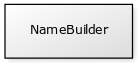
\includegraphics{img/name.png} 
 \end{center}
 \caption{NameBuilder}
\end{figure}


\begin{figure}
 \begin{center}
 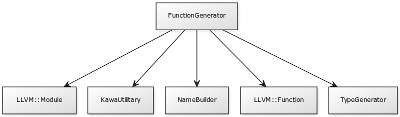
\includegraphics{img/function.png} 
 \end{center}
 \caption{FunctionGenerator}
\end{figure}

\begin{figure}
 \begin{center}
 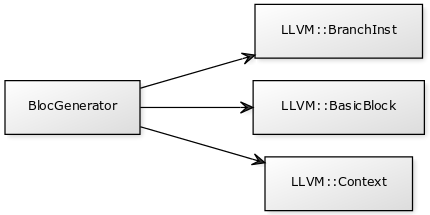
\includegraphics{img/bloc.png} 
 \end{center}
 \caption{BlocGenerator}
\end{figure}

\begin{figure}
 \begin{center}
 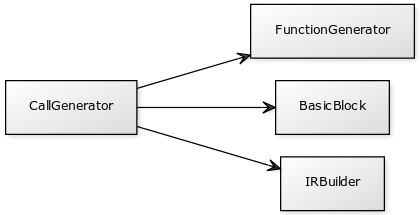
\includegraphics{img/call.png} 
 \end{center}
 \caption{CallGenerator}
\end{figure}

\begin{figure}
 \begin{center}
 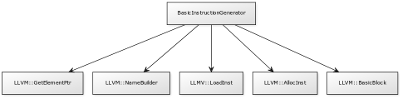
\includegraphics{img/basicInst.png} 
 \end{center}
 \caption{BaiscInstructionFunctionGenerator}
\end{figure}

\begin{figure}
 \begin{center}
 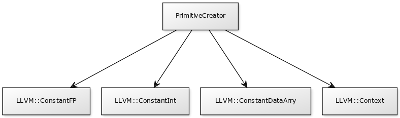
\includegraphics{img/primitive.png} 
 \end{center}
 \caption{PrimitiveCreator}
\end{figure}

\begin{figure}
 \begin{center}
 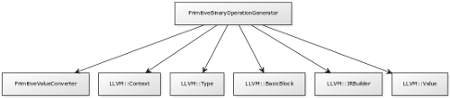
\includegraphics{img/primBin.png} 
 \end{center}
 \caption{PrimitiveBinaryGenerator}
\end{figure}

\begin{figure}
 \begin{center}
 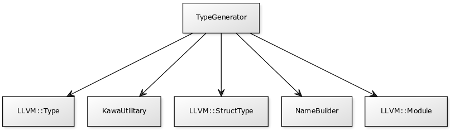
\includegraphics{img/type.png} 
 \end{center}
 \caption{TypeGenerator}
\end{figure}



\end{document}
